\documentclass[12pt,a4paper]{article}
\usepackage[utf8]{inputenc}
\usepackage[T1]{fontenc}
\usepackage{amsmath}
\usepackage{amssymb}
\usepackage{graphicx}
\usepackage[spanish]{babel}
\usepackage[a4paper, margin=2.5cm]{geometry}
\usepackage{enumitem}
\usepackage{hyperref}
\usepackage{comment}

\title{Problemas de Práctica - Semana 6: El Diodo}
\author{Basado en "Circuitos y Dispositivos Electrónicos" de Lluís Prat Viñas, ed.}
\date{\today}

\begin{document}

\maketitle

\section*{Introducción}
Esta selección de 10 problemas corresponde a los temas de la Semana 6 del plan de estudios, cubriendo las secciones 6.1 a 6.3 del libro de referencia. Los problemas están diseñados para reforzar la comprensión de los modelos del diodo y su aplicación en circuitos rectificadores. Se recomienda intentar resolverlos en el orden presentado.

\hrulefill
\vspace{1cm}

\begin{enumerate}[label=\textbf{Problema \arabic*.}, wide, labelindent=0pt]

    \item \textbf{(P6.2 del libro - Dificultad: Baja)} \\
    Dibujar sobre un papel milimetrado en escala lineal, las características I-V de dos diodos a T=300 K, con $I_s = 1 \text{ nA}$ y $I_s = 0.1 \text{ fA}$. (Tomar como escala 1V y 10 nA.)
    \vspace{0.5cm}
    \textit{(Este problema es fundamental para visualizar el efecto de la corriente de saturación inversa $I_s$ en la característica del diodo.)}

    \item \textbf{(P6.1 del libro - Dificultad: Baja)} \\
    A partir de las características I-V del diodo del problema anterior (con $I_s = 0.1 \text{ fA}$), encuentre los parámetros del modelo de tramos lineales ($V_\gamma$ y $R_s$) que mejor lo aproximan en el margen de corrientes de 1 mA a 10 mA.
    \vspace{0.5cm}
    \textit{(Este ejercicio ayuda a comprender cómo se obtiene un modelo simplificado a partir de la curva real del diodo.)}

    \item \textbf{(P6.5 del libro - Dificultad: Media-Baja)} \\
    Encontrar el punto de trabajo ($I_{DQ}, V_{DQ}$) del diodo del circuito de la figura P6.3 resolviendo la ecuación trascendente que resulta al usar el modelo exponencial del diodo con $I_s = 10 \text{ fA}$ (tomar $V_T = 25 \text{ mV}$).

    \begin{center}
        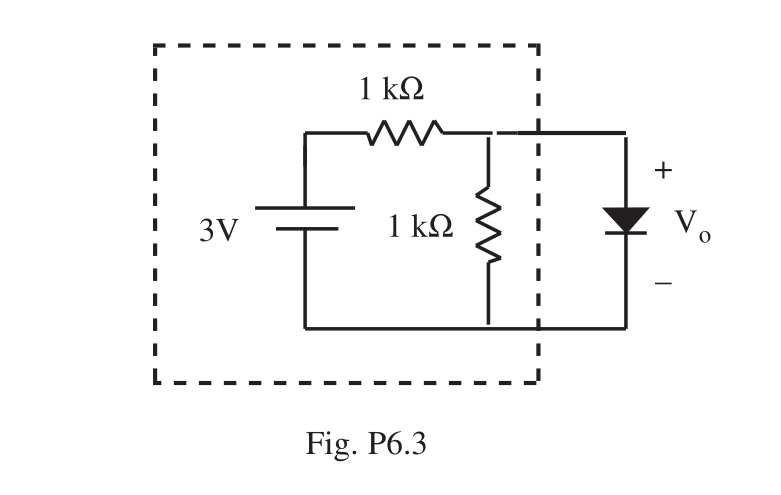
\includegraphics[width=0.4\textwidth]{fig_p6_3.png}
        %\caption*{Figura P6.3 del libro.}
    \end{center}

    \textit{(Este problema introduce el análisis numérico de un circuito simple con diodos, un método potente aunque más complejo que el análisis gráfico.)}

    \item \textbf{(P6.6 del libro - Dificultad: Media-Baja)} \\
    a) Hallar gráficamente la corriente $I_D$ y la tensión $V_D$ en un circuito formado por una fuente constante de 3 V, en serie con una resistencia de 2 $\Omega$, y en serie con un diodo cuyas características son las del diodo del problema P6.2 ($I_s = 0.1 \text{ fA}$). \\
    b) Repetir el análisis anterior de forma numérica sustituyendo el diodo por su modelo de tramos lineales.
    \vspace{0.5cm}
    \textit{(Este ejercicio es excelente para comparar el método gráfico con el modelo de tramos lineales y entender sus respectivas precisiones.)}

    \item \textbf{(P6.7 del libro - Dificultad: Media)} \\
    En el circuito de la figura, la señal de entrada $V_i(t)$ es una onda cuadrada de 10 V de amplitud y 1 ms de período. Se pide: a) Dibujar la forma de onda de la tensión de salida $V_o(t)$. b) Calcular el valor de la componente de continua de la tensión de salida. Supóngase el diodo ideal.

    \begin{center}
        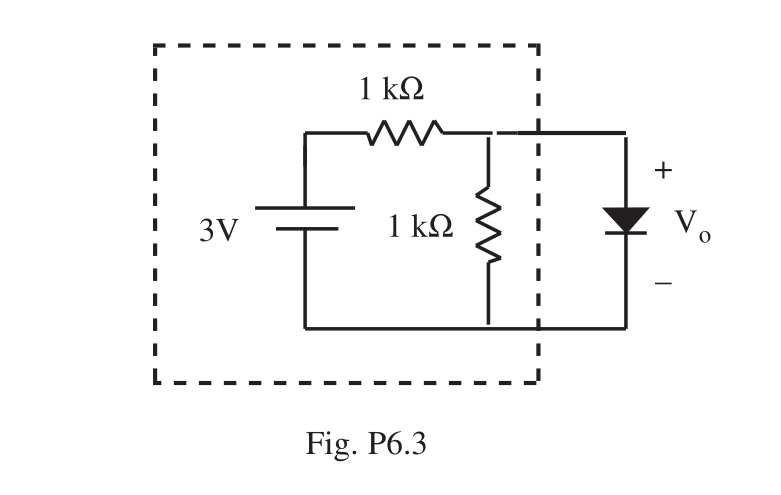
\includegraphics[width=0.4\textwidth]{fig_p6_3.png}
        %\caption*{Figura P6.7 del libro.}
    \end{center}

    \textit{(Este problema aplica el concepto de rectificación a una señal no senoidal, lo cual es importante para generalizar el concepto.)}

    \item \textbf{(P6.10 del libro - Dificultad: Media)} \\
    Para el circuito de la figura P6.10 calcular el margen de tensiones de entrada para que el diodo esté en la región directa, en la región de corte y en la región zener, en función de $V_\gamma$ y $V_Z$. Datos $R_2 = 2R_1 = 2R$.

    \begin{center}
        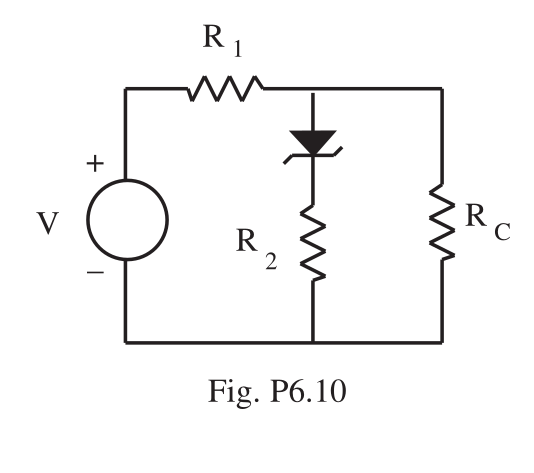
\includegraphics[width=0.4\textwidth]{fig_p6_10.png}
        %\caption*{Figura P6.10 del libro.}
    \end{center}

    \textit{(Aunque introduce el diodo Zener (Semana 7), este problema es una excelente práctica de análisis de estados de un diodo en un circuito más complejo.)}

    \item \textbf{(P6.11 del libro - Dificultad: Media)} \\
    Sea el circuito de la figura P6.11, donde los diodos pueden representarse según el modelo de tramos lineales con $V_\gamma = 0.6 \text{ V}$, $V_Z = -4 \text{ V}$, $R_Z = 10 \, \Omega$ y $R_s = 1 \, \Omega$. Se pide: a) Determinar las condiciones para que los diodos estén en directa, en corte y en ruptura. b) Dibujar la gráfica $V_o - V_i$. c) Dibujar la onda de salida cuando la señal de entrada es una onda triangular de 10 V de pico.

    \begin{center}
        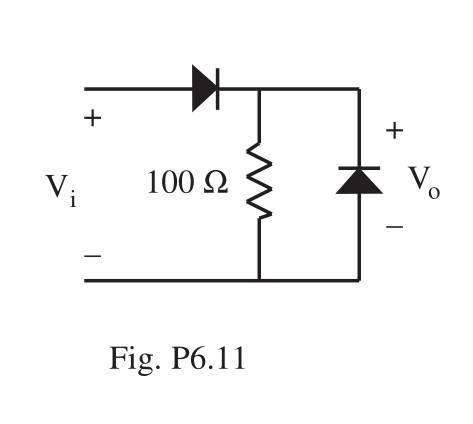
\includegraphics[width=0.3\textwidth]{fig_p6_11.png}
        %\caption*{Figura P6.11 del libro.}
    \end{center}

    \textit{(Este es un problema muy completo sobre circuitos recortadores con dos niveles.)}

    \item \textbf{(P6.12 del libro - Dificultad: Media-Alta)} \\
    En el rectificador de doble onda de la figura 6.17b, dibujar la forma de onda en la carga $R_L$ suponiendo que $v_g$ es 10sen($\omega t$), $V_\gamma = 0.7 \text{ V}$, $R_s = 5 \, \Omega$ y $R_L = 1 \text{ k}\Omega$.
    \vspace{0.5cm}
    \textit{(Este ejercicio requiere analizar cuidadosamente el funcionamiento del puente rectificador, considerando la caída de tensión en los diodos.)}

    \item \textbf{(P6.13 del libro - Dificultad: Media-Alta)} \\
    Dado el circuito de la figura P6.13: a) Describir su funcionamiento. b) Si para los diodos se toma $V_\gamma = 0.7 \text{ V}$ y $R_s = 5 \, \Omega$, dibujar la forma de onda de la tensión de salida del circuito $V_o$ para una entrada $V_i = V_p \text{sen}(\omega t)$.

    \begin{center}
        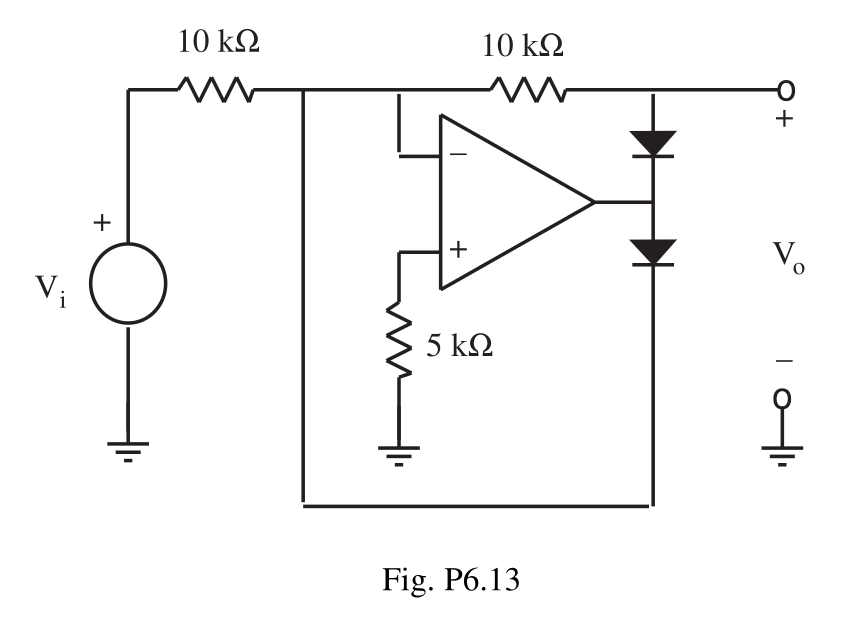
\includegraphics[width=0.4\textwidth]{fig_p6_13.png}
        %\caption*{Figura P6.13 del libro.}
    \end{center}

    \textit{(Este circuito es un rectificador de precisión. Analizarlo requiere entender la interacción entre el diodo y el amplificador operacional.)}

    \item \textbf{(P6.17 del libro - Dificultad: Alta)} \\
    En el circuito rectificador de media onda con filtro de condensador suponer $V_i = 10 \text{sen}(\omega t)$ con $f=50 \text{ Hz}$, el diodo ideal y la resistencia de carga $R_L$ de 100 $\Omega$. Se pide: a) ¿Cuál debe ser el valor de C para que el rizado sea de 0.5 V? b) Estimar el tiempo de conducción del diodo. c) Estimar la carga que ha cedido el condensador a $R_L$ durante el tiempo en que el diodo ha permanecido cortado. d) ¿Cuál será la corriente por el diodo durante la recarga del condensador si dicha corriente fuera constante durante el tiempo de conducción del diodo?
    \vspace{0.5cm}
    \textit{(Este es un problema de diseño y análisis completo de una de las aplicaciones 
    más importantes del diodo: la fuente de alimentación con filtro capacitivo.)}

\end{enumerate}

\end{document}

%%% Imágenes requeridas (deben estar en la misma carpeta que el .tex)
%%% fig_p6_3.png
%%% fig_p6_7.png
%%% fig_p6_10.png
%%% fig_p6_11.png
%%% fig_p6_13.png